% --- 章节开始 ---
\newpage
\section*{第二章\quad 相关理论和技术}
\label{chap:related}
\setcounter{section}{2} \setcounter{subsection}{0}
\addcontentsline{toc}{section}{第二章\quad 相关理论和技术}


本章将说明本文研究涉及的核心理论与关键技术。首先,介绍推荐系统的基本概念、分类及常用评价指标,并重点阐述图神经网络(GNN)基本原理及其在异构图与超图推荐中的应用机制;其次,概述联邦学习的架构分类,剖析模型压缩策略在联邦场景下的应用;最后,介绍对比学习范式和其在图结构视图增强及缓解数据稀疏性方面的应用。

\subsection{推荐系统基础}
互联网数据的指数级增长使得用户面临"信息过载"问题。推荐系统(Recommender System, RS)作为解决这一问题的核心技术手段,已广泛应用于电子商务、社交媒体及内容分发平台\cite{zhang2024social}。

\subsubsection{推荐系统的目标}
推荐系统的核心目标是在没有明确用户检索指令的情况下,通过分析用户的历史行为数据(如点击、购买、评分)及辅助属性信息,挖掘用户潜在的兴趣偏好。从数学建模的角度来看,推荐任务通常被形式化为\textbf{矩阵补全(Matrix Completion)}或\textbf{链接预测(Link Prediction)}问题。

\textbf{1. 矩阵补全视角:}

令 $\mathcal{U} = \{u_1, u_2, \dots, u_m\}$ 表示包含 $m$ 个用户的集合,$\mathcal{V} = \{v_1, v_2, \dots, v_n\}$ 表示包含 $n$ 个物品的集合。用户与物品之间的交互行为可以表示为一个交互矩阵 $\mathbf{Y} \in \mathbb{R}^{m \times n}$,其中矩阵元素 $y_{uv}$ 定义如下:
\begin{equation}
y_{uv} = \begin{cases} 
1, & \text{如果用户 } u \text{ 与物品 } v \text{ 存在观测交互} \\
0, & \text{否则(未观测数据)}
\end{cases}
\end{equation}
在此视角下,推荐系统的目标是利用已知观测数据去拟合参数,推断矩阵 $\mathbf{Y}$ 中未观测项(即 $0$ 元素)的真实评分 $\hat{y}_{uv}$。

\textbf{2. 链接预测视角:}

上述交互矩阵 $\mathbf{Y}$ 可等价地映射为一个\textbf{用户-物品二部图(User-Item Bipartite Graph)} $\mathcal{G} = (\mathcal{N}, \mathcal{E})$。其中,节点集 $\mathcal{N} = \mathcal{U} \cup \mathcal{V}$ 包含了所有的用户和物品,边集 $\mathcal{E} = \{(u, v) | y_{uv} = 1\}$ 则表示观测到的交互关系。
在此视角下,推荐任务转化为\textbf{链接预测}问题:即根据图中已有的拓扑结构和节点特征,预测在用户节点 $u$ 和物品节点 $v$ 之间是否存在一条潜在的边(Link),并计算其连接概率 $p(u, v)$。根据链接概率判断用户和物品之间是否存在真实关系\cite{he2020lightgcn}。

无论是预测矩阵评分 $\hat{y}_{uv}$ 还是预测连接概率 $p(u, v)$,最终系统都会根据预测值对物品进行 Top-K 排序并推荐给目标用户。

\subsubsection{推荐系统的分类}
根据算法原理及数据利用方式的不同,现有的推荐系统主要可以分为以下几种常见类型:

\begin{enumerate}[wide, labelwidth=!, labelindent=\parindent]
    % --- (1) 协同过滤 ---
    \item \textbf{协同过滤推荐(Collaborative Filtering, CF)}
    
    协同过滤是推荐系统发展历程中最经典且应用最广泛的方法之一。其核心思想基于“群体智慧”,即利用用户的历史行为数据(如点击、购买、评分)来挖掘用户或物品之间的相关性,主要分为基于用户的协同过滤和基于物品的协同过滤两种形式。
    
    \begin{enumerate}[wide, labelwidth=!, labelindent=\parindent]
        \item \textbf{基于用户的协同过滤(UserCF):} UserCF 的基本假设是"兴趣相似的用户往往喜欢相同的物品"。其算法流程首先是通过历史行为计算目标用户与其他用户的相似度,找到与目标用户兴趣最相近的邻居群体(Nearest Neighbors),然后将邻居群体偏好但目标用户尚未交互的物品进行推荐。
        
        如图 \ref{fig:usercf} 所示:用户 A 和用户 C 都对物品 A(篮球)和物品 C(足球)表现出兴趣,通过相似度计算可认为两者具有相似的偏好。由于用户 C 还交互过物品 D(电子产品),因此推断用户 A 也可能对物品 D 感兴趣。

        \item \textbf{基于物品的协同过滤(ItemCF):} 与 UserCF 不同,ItemCF 从物品的角度出发,其基本假设是"用户往往喜欢与其过去喜欢的物品相似的物品"。该算法首先计算物品之间的相似度,当用户对某物品产生行为后,系统会向其推荐与该物品相似度较高的其他物品。

        如图 \ref{fig:itemcf} 所示:物品 A(篮球)和物品 C(足球)因被多位共同用户交互而被判定为相似物品。当系统检测到用户 A 对物品 A 有历史交互时,便会基于物品间的相似性,将物品 C 推荐给用户 A。
\end{enumerate}

\begin{figure}[H]
    \centering
    \includegraphics[width=0.75\textwidth]{images/usecf.png} 
    \caption{UserCF 算法原理示意图}
    \label{fig:usercf}
\end{figure}

\begin{figure}[H]
    \centering
    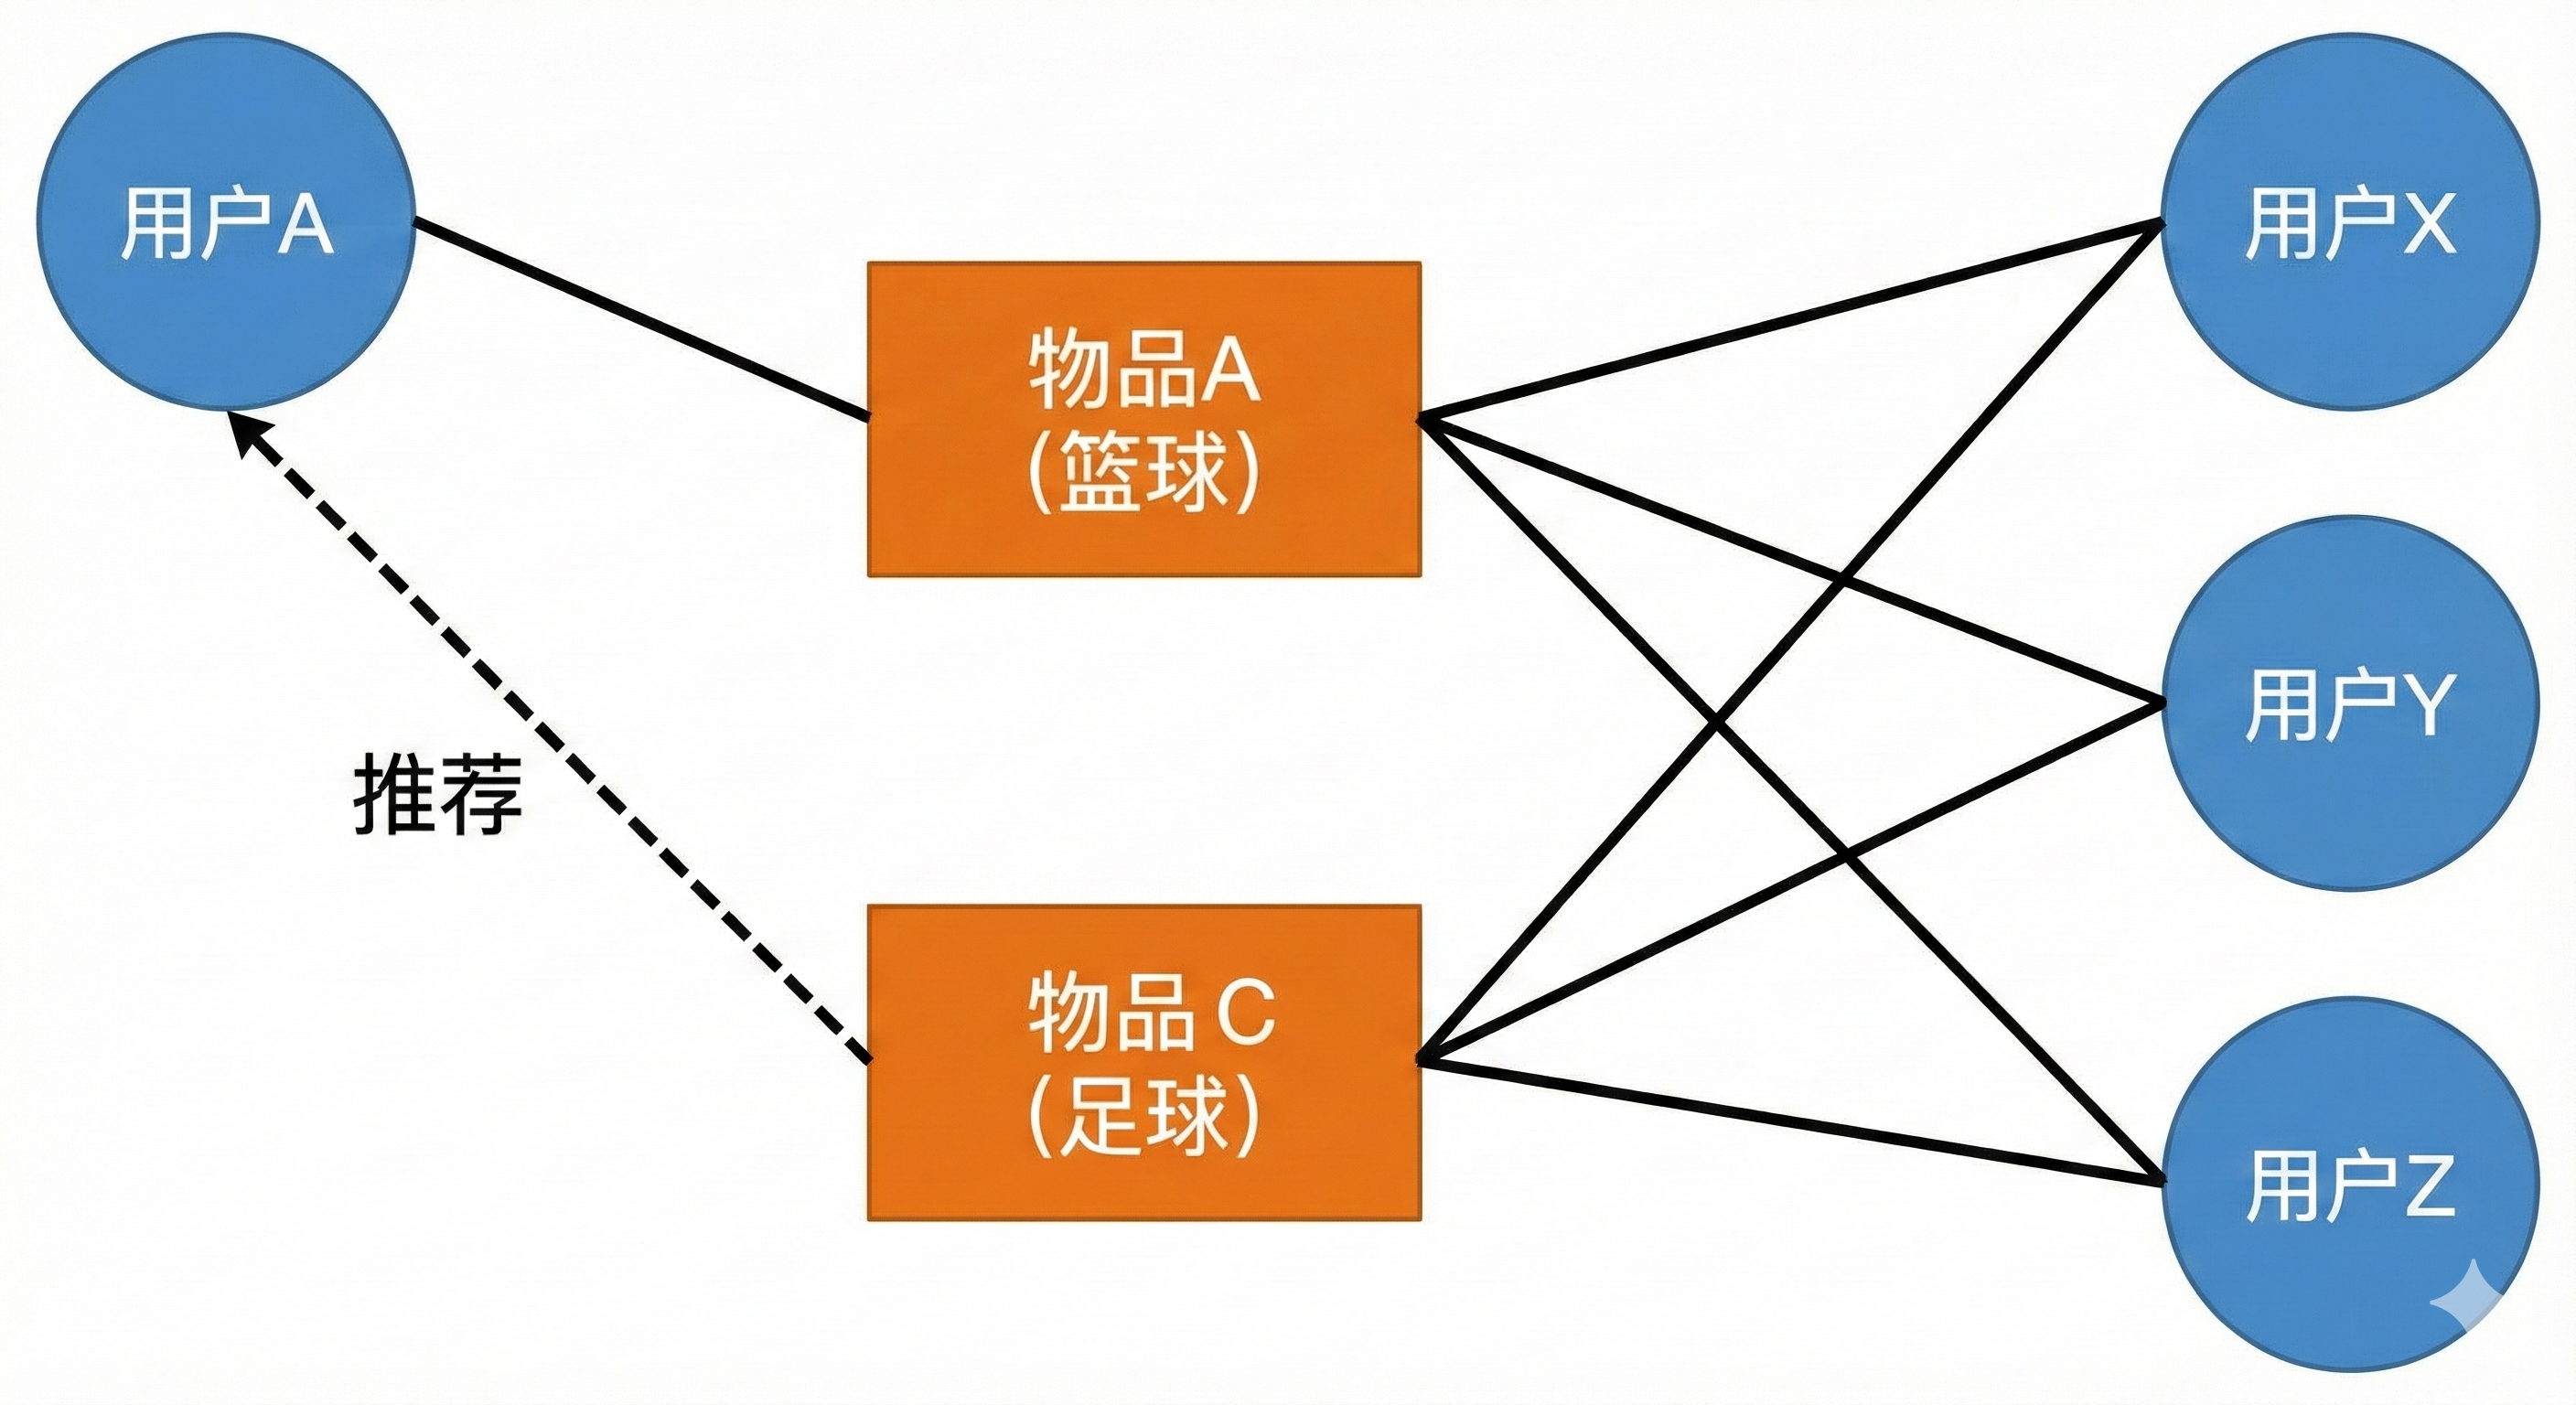
\includegraphics[width=0.75\textwidth]{images/CF.png}
    \caption{ItemCF 算法原理示意图}
    \label{fig:itemcf}
\end{figure}

    \textbf{优缺点分析:} 协同过滤算法具有模型通用性强、无需领域知识等优点。然而,其严重依赖历史交互数据,在面对\textbf{数据稀疏(Data Sparsity)}问题时推荐质量会明显下降;同时,对于无历史行为的新用户或新物品,存在严重的\textbf{冷启动(Cold Start)}问题\cite{qiao2018coldstart}。

    % --- (2) 矩阵分解 ---
    \item \textbf{矩阵分解方法(Matrix Factorization, MF)}
    
    矩阵分解是协同过滤算法在隐语义挖掘方向的延伸。其核心原理是将高维稀疏的用户-物品评分矩阵 $\mathbf{Y}$ 分解为两个低维的稠密矩阵:用户潜在特征矩阵 $\mathbf{P}$ 和物品潜在特征矩阵 $\mathbf{Q}$。通过将用户和物品映射到同一个低维隐向量空间,利用向量内积来预测用户对物品的评分或偏好程度。
    
    原理如图 \ref{fig:mf} 所示。

\begin{figure}[H]
    \centering
    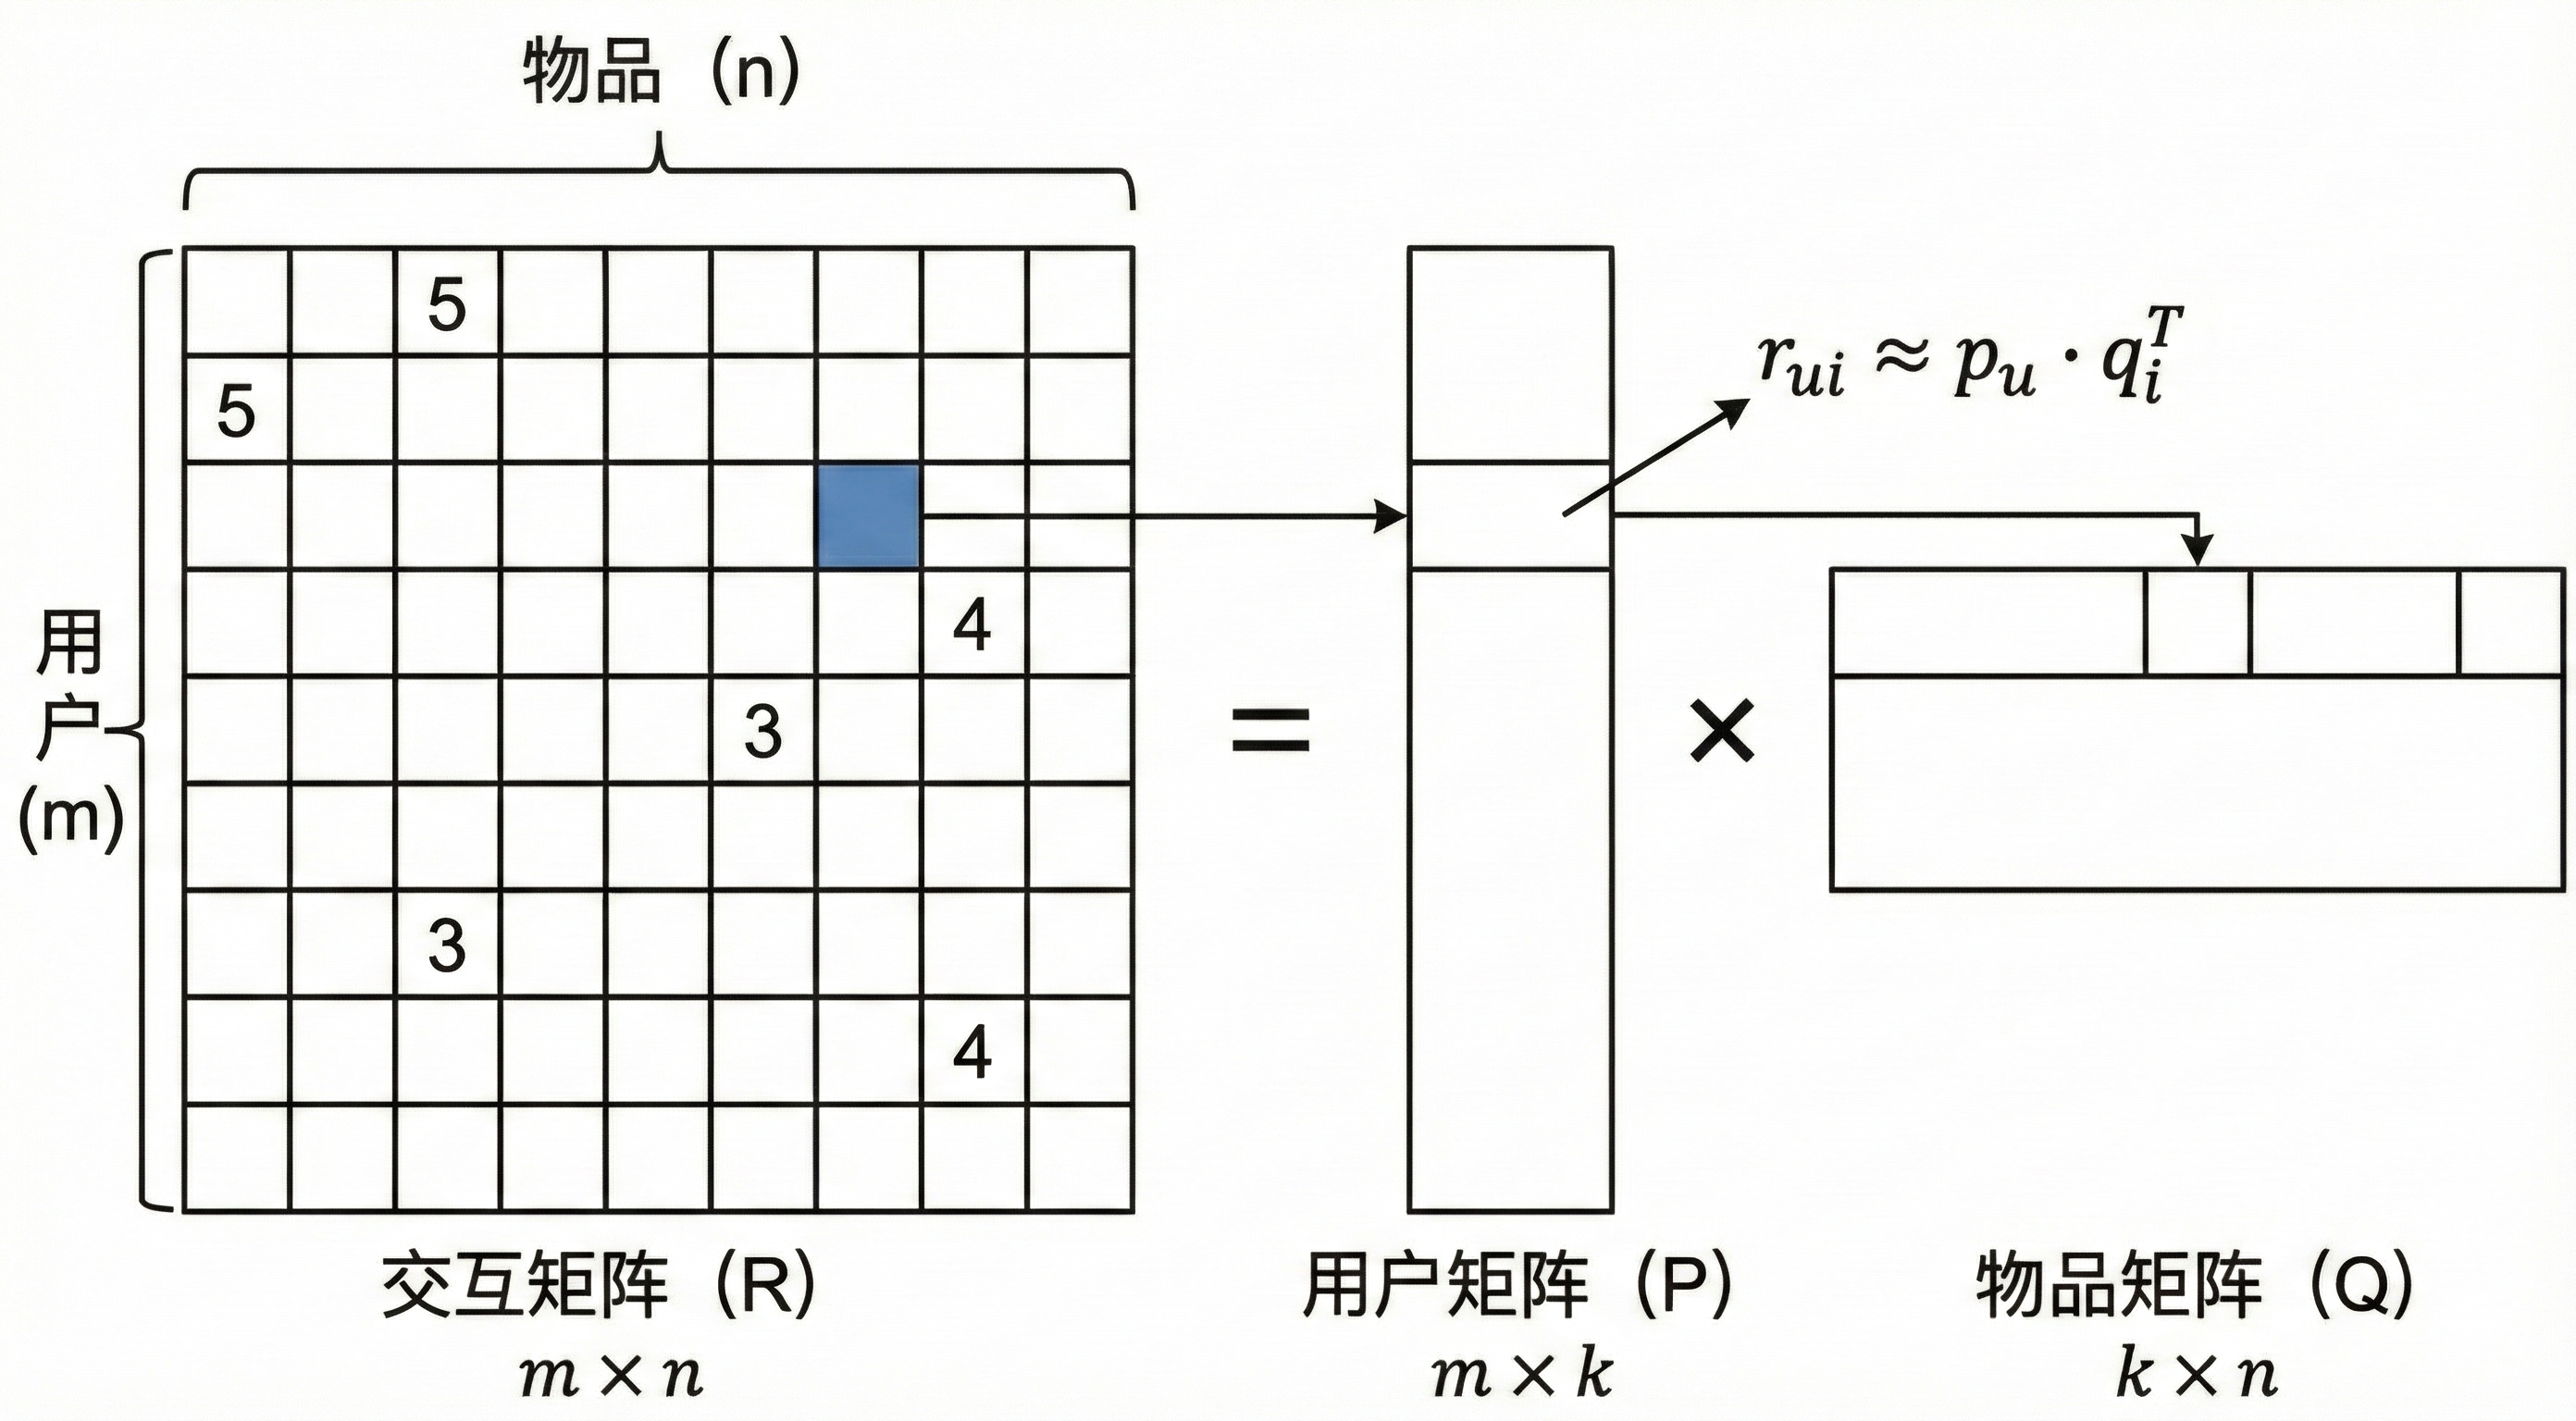
\includegraphics[width=0.8\textwidth]{images/matrix.png}
    \caption{矩阵分解(MF)示意图}
    \label{fig:mf}
\end{figure}

    % --- (3) 深度学习 ---
    \item \textbf{深度学习方法}
    
    深度学习技术的发展推动了神经网络在推荐系统中的应用。常见的方法包括:
    \begin{enumerate}
        \item \textbf{神经协同过滤(NCF):} 利用多层感知机(MLP)替代矩阵分解中的简单内积操作,以拟合用户与物品之间复杂的非线性交互函数。
        \item \textbf{序列推荐:} 利用循环神经网络(RNN)、Transformer 或 BERT 等模型建模用户行为的时间序列特征,捕捉用户兴趣的动态演化\cite{zhao2024multiinterest}。
    \end{enumerate}

    % --- (4) 基于图的推荐 ---
    \item \textbf{基于图的推荐系统}
    
    因为用户-物品交互数据天然具备图结构特性(即用户和物品可视为节点,交互行为视为边),基于图的推荐方法通过在图结构上来挖掘高阶协同信号。相较于传统方法,图方法能够利用多跳邻居信息,从而更准确地建模用户偏好\cite{he2020lightgcn, mao2021ultragcn}。关于该类方法的详细原理与演进,将在 \ref{sec:gnn_rec} 小节中进行详细阐述。
\end{enumerate}

\subsubsection{推荐系统常用的衡量指标}
为了全面、客观地评估推荐算法的性能,验证模型在 Top-K 推荐场景下的有效性,业界中常用的评估指标有:召回率(Recall)、归一化折损累计增益(NDCG)、曲线下面积(AUC)以及命中率(Hit Ratio)等。各指标的具体定义与计算公式如下:

\begin{enumerate}[label=(\arabic*)]
    \item \textbf{召回率(Recall@K)}
    
    Recall@K 是衡量推荐系统检索能力的核心指标,主要考察模型在 Top-K 推荐列表中覆盖用户真实感兴趣项目的比例。该指标关注的是“查全率”,即用户喜欢的物品有多少被模型成功找回。其数值越高,表明模型遗漏的正样本越少,推荐覆盖面越广。对于测试集中的用户集合 $\mathcal{U}$,其计算公式如式 \eqref{eq:recall} 所示:
    \begin{equation}
        \text{Recall}@K = \frac{1}{|\mathcal{U}|} \sum_{u \in \mathcal{U}} \frac{|\mathcal{R}_u \cap \mathcal{P}_u@K|}{|\mathcal{R}_u|}
        \label{eq:recall}
    \end{equation}
    式中,$\mathcal{R}_u$ 表示测试集中用户 $u$ 实际交互过的相关项目集合(Ground Truth);$\mathcal{P}_u@K$ 表示模型为用户 $u$ 生成的前 $K$ 个推荐项目列表;$|\cdot|$ 表示集合中元素的个数。

    \item \textbf{归一化折损累计增益(NDCG@K)}
    
    NDCG(Normalized Discounted Cumulative Gain)是评估推荐列表排序质量的重要指标。与 Recall 不同,NDCG 不仅关注模型是否推荐了正确的物品,还对物品在列表中的位置极其敏感。根据位置折损原则,排名越靠前的项目对最终分数的贡献越大。NDCG@K 的值介于 0 到 1 之间,值越高代表排序效果越符合用户偏好。其计算过程如式 \eqref{eq:ndcg} 所示:
    \begin{equation}
        \text{NDCG}@K = \frac{1}{|\mathcal{U}|} \sum_{u \in \mathcal{U}} \frac{\text{DCG}_u@K}{\text{IDCG}_u@K}
        \label{eq:ndcg}
    \end{equation}
    其中 $\text{DCG}_u@K$ 为折损累计增益,计算公式为 $\sum_{i=1}^{K} \frac{2^{rel_i} - 1}{\log_2(i+1)}$,$rel_i$ 表示第 $i$ 个位置的项目的相关性(在隐式反馈中,交互为1,否则为0);$\text{IDCG}_u@K$ 为理想状态下的最大累计增益,用于进行归一化处理。

    \item \textbf{曲线下面积(AUC)}
    
    AUC(Area Under the Curve)即 ROC 曲线下的面积,在推荐系统中常用于评估模型对正负样本的排序区分能力。从概率角度解释,AUC 代表了随机抽取一个正样本(用户喜欢的)和一个负样本(用户不喜欢的),模型对正样本的预测得分高于负样本得分的概率。AUC = 0.5 表示模型效果等同于随机猜测,AUC 越接近 1 表示模型的排序能力越强。其计算公式如式 \eqref{eq:auc} 所示:
    \begin{equation}
        \text{AUC} = \frac{1}{|\mathcal{U}|} \sum_{u \in \mathcal{U}} \frac{1}{|\mathcal{P}_u||\mathcal{N}_u|} \sum_{i \in \mathcal{P}_u} \sum_{j \in \mathcal{N}_u} \mathbb{I}(\hat{y}_{ui} > \hat{y}_{uj})
        \label{eq:auc}
    \end{equation}
    式中,$\mathcal{P}_u$ 和 $\mathcal{N}_u$ 分别表示用户 $u$ 的正样本集合和负样本集合;$\hat{y}_{ui}$ 和 $\hat{y}_{uj}$ 分别为模型对正样本 $i$ 和负样本 $j$ 的预测分数;$\mathbb{I}(\cdot)$ 为指示函数,当条件成立时取值为 1,否则为 0。

    \item \textbf{命中率(Hit@K)}
    
    Hit@K(Hit Ratio)是一种直观的准确性指标,用于衡量推荐列表 Top-K 中是否至少包含一个用户实际交互过的正样本。该指标通常用于留一法(Leave-One-Out)评估场景中。Hit@K 关注的是推荐结果的“存在性”,即模型是否“击中”了用户的兴趣点。其计算公式如式 \eqref{eq:hit} 所示:
    \begin{equation}
        \text{Hit}@K = \frac{1}{|\mathcal{U}|} \sum_{u \in \mathcal{U}} \mathbb{I}(|\mathcal{R}_u \cap \mathcal{P}_u@K| \geq 1)
        \label{eq:hit}
    \end{equation}
    式中,$\mathcal{R}_u$ 为用户 $u$ 的真实正样本集合,$\mathcal{P}_u@K$ 为模型推荐的前 $K$ 个项目。如果交集非空,说明推荐列表中包含至少一个正样本,指示函数记为 1,否则为 0。
\end{enumerate}

\subsection{图神经网络推荐技术}
\label{sec:gnn_rec}

\subsubsection{图神经网络(GNN)基本原理}
传统的协同过滤方法(如矩阵分解 MF)主要通过点积将用户和物品映射到同一潜在空间,这种方法本质上只建模了用户与物品的一阶线性关系,难以捕捉复杂的非线性结构信息。图神经网络(Graph Neural Networks, GNNs)通过在图结构上执行消息传递(Message Passing)机制,有效地解决了上述问题\cite{wu2021fedgnn, he2020lightgcn}。

GNN 的核心思想是利用图的拓扑结构,迭代地聚合邻居节点的特征信息,从而更新中心节点的表示。在推荐场景下,其基本原理主要包含以下三个步骤:

\textbf{(1)图结构定义与初始化}:定义用户集合 $\mathcal{U}$ 和物品集合 $\mathcal{V}$,交互图表示为 $\mathcal{G} = (\mathcal{U} \cup \mathcal{V}, \mathcal{E})$,其中 $\mathcal{E}$ 为边集。首先,为每个用户 $u$ 和物品 $v$ 初始化低维稠密向量(Embedding),记为 $\mathbf{e}_u^{(0)}$ 和 $\mathbf{e}_v^{(0)}$,作为第 0 层的输入特征。

\textbf{(2)消息传递与聚合}:消息传递是 GNN 的核心。在第 $l$ 层网络中,目标节点会收集其邻居节点的信息。对于用户节点 $u$,其聚合过程可以形式化为:
\begin{equation}
    \mathbf{m}_{\mathcal{N}_u}^{(l)} = \text{AGGREGATE}^{(l)} \left( \{ \mathbf{e}_i^{(l-1)} : i \in \mathcal{N}_u \} \right) 
    \label{eq:gnn_agg}
\end{equation}
其中,$\mathcal{N}_u$ 表示用户 $u$ 的邻居节点集合(即交互过的物品),$\mathbf{e}_i^{(l-1)}$ 是邻居节点在上一层的特征表示,$\text{AGGREGATE}(\cdot)$ 是聚合函数,常见的形式包括均值聚合(Mean Pooling)、最大值聚合(Max Pooling)或加权求和等。

\textbf{(3)特征更新与高阶协同}:在聚合了邻居信息后,模型结合节点自身的当前状态进行更新,生成新的节点表示:
\begin{equation}
    \mathbf{e}_u^{(l)} = \text{UPDATE}^{(l)} \left( \mathbf{e}_u^{(l-1)}, \mathbf{m}_{\mathcal{N}_u}^{(l)} \right)
    \label{eq:gnn_update}
\end{equation}
通过堆叠 $L$ 层 GNN 网络,节点 $u$ 的最终表示 $\mathbf{e}_u^{(L)}$ 实际上融合了其 $L$ 跳(L-hop)邻居的信息。这种机制使得模型能够显式地编码高阶协同信号(High-order Connectivity)。例如,通过“用户A-物品1-用户B-物品2”的路径,模型可以挖掘出具有相似偏好的潜在用户群体,缓解了数据稀疏性问题,提升了推荐的准确性\cite{wang2019kgat}。

\begin{figure}[H]
    \centering
    \includegraphics[width=0.9\textwidth]{images/图神经网络.png} 
    \caption{图神经网络算法原理示意图}
    \label{fig:gnn}
\end{figure}

\subsubsection{同构图和异构图}

\begin{enumerate}
    \item \textbf{同构图(Homogeneous Graph)}:
    
    同构图是图结构中最简单的形式,图中所有的顶点都属于同一类型,并且所有的边也都属于同一类型。同构图示例如图 \ref{fig:homo_graph} 所示,图中的顶点具有相同的语义和属性集合,边也具有相同的语义和属性集合。
    
    用数学语言描述,设图 $G=(V, E)$,其中 $V$ 是顶点的集合,$E$ 是边的集合。对于任意的顶点 $u, v \in V$,它们具有相同的类型;对于任意的边 $(u, v) \in E$,这些边也具有相同的类型。
\end{enumerate}

\begin{figure}[H]
    \centering
    \includegraphics[width=0.6\textwidth]{images/同构图.png} 
    \caption{同构图示意图}
    \label{fig:homo_graph}
\end{figure}

\begin{enumerate}
    \item \textbf{异构图(Heterogeneous Graph)}:
    
    异构图是指图中存在多种类型的节点和边,每种类型可能代表不同的实体或关系。在异构图中,节点和边的不同属性赋予了图更丰富的语义信息\cite{yan2024fedhgnn}。
    
    形式化地,给定异构图 $\mathcal{G} = (\mathcal{V}, \mathcal{E}, \mathcal{A}, \mathcal{R})$,其中 $\mathcal{V}$ 是顶点集,$\mathcal{E}$ 是边集,$\mathcal{A}$ 是顶点类型集合,$\mathcal{R}$ 是边类型集合。异构图包含两个映射函数:
    \begin{enumerate}
        \item 顶点类型映射函数 $\phi: \mathcal{V} \rightarrow \mathcal{A}$,将顶点映射到一个顶点类型集合 $\mathcal{A}$ 中的某一类型;
        \item 边类型映射函数 $\psi: \mathcal{E} \rightarrow \mathcal{R}$,将边映射到一个边类型集合 $\mathcal{R}$ 中的某一类型。
    \end{enumerate}
    且满足 $|\mathcal{A}| > 1$ 或者 $|\mathcal{R}| > 1$(即至少存在两种顶点类型或者两种边类型)。
\end{enumerate}
现实世界的网络结构往往呈现出高度的复杂性,包含多种类型的实体及它们之间错综复杂的交互关系。相比于传统的单一视图建模,采用异构图能够完整保留数据的结构异质性(Structural Heterogeneity),从而更精准地捕捉实体间深层次的语义关联与依赖信息。

\subsubsection{基于元路径的推荐}
在异构信息网络(HIN)中,由于节点和边类型的多样性,直接应用传统的同构图算法难以捕捉复杂的语义信息,为了解决这个问题,Sun 等人提出了元路径(Meta-path)的概念。

对于给定网络模式 $T_G = (\mathcal{A}, \mathcal{R})$,元路径 $\mathcal{P}$ 是定义在网络模式上形如 $\mathcal{A}_1 \xrightarrow{\mathcal{R}_1} \mathcal{A}_2 \xrightarrow{\mathcal{R}_2} \dots \xrightarrow{\mathcal{R}_l} \mathcal{A}_{l+1}$ 的序列。其中,$\mathcal{A}_i \in \mathcal{A}$ 表示节点类型,$\mathcal{R}_i \in \mathcal{R}$ 表示连接节点类型 $\mathcal{A}_i$ 与 $\mathcal{A}_{i+1}$ 的关系。元路径定义了起始节点类型 $\mathcal{A}_1$ 与目标节点类型 $\mathcal{A}_{l+1}$ 之间的一种复合关系 $R = \mathcal{R}_1 \circ \mathcal{R}_2 \circ \dots \circ \mathcal{R}_l$。

对于给定的元路径 $\mathcal{P}$,用户节点 $u$ 的基于元路径的邻居集合 $\mathcal{N}_u^{\mathcal{P}}$ 包含了所有通过该路径与 $u$ 建立连接的节点。在推荐模型的特征学习阶段,模型通过以下聚合函数(Aggregation Function)生成用户在该特定语义下的嵌入表示(Embedding):
\begin{equation}
    \mathbf{h}_u^{\mathcal{P}} = \text{AGGREGATE}_{\mathcal{P}} \left( \left\{ \mathbf{h}_v \mid v \in \mathcal{N}_u^{\mathcal{P}} \right\} \right)
\end{equation}
其中,$\mathbf{h}_v$ 表示邻居节点的初始特征向量,$\text{AGGREGATE}(\cdot)$ 通常采用平均池化(Mean Pooling)或注意力机制(Attention Mechanism)\cite{wang2019han}。例如,在“User-Movie-User”路径下,聚合操作实际上是在学习“与其观看历史相似的其他用户”的特征分布,从而捕捉协同过滤语义\cite{li2023metapath}。

\begin{figure}[H]
    \centering
    \includegraphics[width=0.75\textwidth]{images/元路径.png}
    \caption{异构图与元路径示意图}
    \label{fig:meta_path}
\end{figure}

\subsection{联邦学习概述}

联邦学习是由谷歌(Google)于 2016 年首次提出的一种新兴分布式机器学习范式,旨在打破"数据孤岛"并保护用户隐私\cite{li2025openfgl}。

其核心理念在于"\textbf{数据不动模型动}",即在不共享原始数据、保护数据隐私的同时,利用分布在不同客户端(Clients)的数据协同训练出一个全局模型。联邦学习通常采用\textbf{客户端-服务器(Client-Server)}架构\cite{deng2023survey}。

一轮标准的联邦学习训练包含以下四个步骤:

\begin{enumerate}
    \item \textbf{梯度发送(本地训练)} : 参与训练的客户端首先接收服务器下发的初始全局模型,利用本地数据进行训练,得到本地模型。训练完成后,客户端将计算出的加密梯度上传至服务器。

    \item \textbf{安全聚合} : 服务器收到各个参与客户端上传的加密梯度后,利用聚合算法(如安全聚合)对梯度进行汇总处理,从而更新全局模型。

    \item \textbf{模型返回} : 服务器将更新后的全局模型发送回所有参与训练的客户端。

    \item \textbf{模型更新} : 参与客户端收到最新的全局模型后,用其更新本地模型,准备进行下一轮训练。
\end{enumerate}

上述步骤不断迭代,直至模型收敛,最终获得可用的全局模型。

\begin{figure}[H]
    \centering
    \includegraphics[width=0.8\textwidth]{images/联邦推荐图.jpg} 
    \caption{联邦学习架构示意图}
    \label{fig:fl_overview}
\end{figure}

同时根据参与方数据的分布特性(即数据样本与特征空间的重叠情况),联邦学习通常被分为横向联邦学习、纵向联邦学习和联邦迁移学习三类\cite{guo2024fedgnn}。
\begin{enumerate}
    \item \textbf{横向联邦学习(Horizontal FL):} 主要适用于参与方数据特征空间重叠较多、但样本空间重叠较少的场景。这意味着不同参与方拥有相似的业务场景或数据结构,但服务于不同的用户群体。
    
    例如:不同的高校电子图书馆两者拥有相似的数据特征(均包含学生的论文下载记录、检索关键词、浏览时长等),但各自服务于不同的学生群体。通过横向联邦学习,双方可以联合利用更大规模的阅读行为数据,训练出泛化能力更强的论文推荐模型。
\end{enumerate}

\begin{figure}[H]
    \centering
    \includegraphics[width=0.8\textwidth]{images/横向联邦学习.png} 
    \caption{横向联邦学习示意图}
    \label{fig:horz_fl}
\end{figure}

\begin{enumerate}
    \item \textbf{纵向联邦学习(Vertical FL):} 主要适用于参与方数据样本空间重叠较多、但特征空间重叠较少的场景。这种情况常见于同一地区的不同机构之间,它们拥有同一批用户,但掌握该用户不同维度的属性数据。
    
    例如:一所高校的电子图书馆与该校的科研管理系统。两者服务于同一批师生用户(样本相同),但图书馆掌握用户的论文下载与阅读记录,而科研系统掌握用户的论文发表情况与课题申报信息。通过纵向联邦学习,可以将用户的"阅读输入"与"科研输出"数据相结合,构建画像更立体的推荐模型,向用户推荐更符合其科研产出方向的文献\cite{wang2025p4gcn}。
\end{enumerate}

\begin{figure}[H]
    \centering
    \includegraphics[width=0.8\textwidth]{images/纵向联邦学习.png} 
    \caption{纵向联邦学习示意图}
    \label{fig:vert_fl}
\end{figure}

\begin{enumerate}
    \item \textbf{迁移联邦学习(Transfer FL):} 主要适用于参与方数据样本空间与特征空间均存在较大差异,且少量重叠的场景,解决单边数据稀缺或标签不足的问题。 
    
    例如:英文计算机科学(CS)论文数据库与新兴的中文生物医学论文平台。两者的用户群体和数据特征均存在巨大差异。通过联邦迁移学习,可以在两者仅有的交叉学科(如生物信息学)重叠数据上进行对齐,将CS数据库中成熟的引文图谱结构知识迁移到生物医学平台,解决新兴平台因数据稀缺导致的推荐冷启动问题\cite{li2025fedcsr, chen2024fedgcdr}。
\end{enumerate}

\begin{figure}[H]
    \centering
    \includegraphics[width=0.8\textwidth]{images/迁移学习.png} 
    \caption{联邦迁移学习示意图}
    \label{fig:trans_fl}
\end{figure}

\subsection{对比学习}
对比学习(Contrastive Learning)是一种自监督学习方法,其核心思想是通过构造正负样本对,让模型学会区分相似与不相似的样本,从而获得具有判别性的表征\cite{crad2024multiview}。在推荐系统面临数据稀疏(Data Sparsity)和冷启动(Cold Start)问题时,对比学习能够利用数据自身的结构信息或增强视图构建辅助监督信号,从而在缺乏人工标注或交互记录的情况下,依然能学习出高质量的特征表示\cite{zhang2024ifedrec}。

对比学习的基本流程如下:对于一个输入样本 $x$(在推荐场景中可以是用户、物品或交互子图),通过两种不同的数据增强策略 $\mathcal{T}_1$ 和 $\mathcal{T}_2$ 分别生成两个增强视图 $\tilde{x}_i = \mathcal{T}_1(x)$ 和 $\tilde{x}_j = \mathcal{T}_2(x)$,它们被视为一对正样本(Positive Pair);同时,从同一个批次(Batch)的其他样本增强视图中采样,构建与当前视图语义相反的“负样本对”(Negative Pair)\cite{yu2022simgcl}。所有视图经过同一个编码器 $f(\cdot)$(如 GNN 或 Transformer)映射到特征空间,再经过投影头得到表示向量 $z_i = g(f(\tilde{x}_i))$ 和 $z_j = g(f(\tilde{x}_j))$。优化的目标是拉近正样本对在特征空间中的距离,同时推远负样本对的距离。在此过程中,最常用的损失函数是归一化温度缩放的对比损失(Normalized Temperature-scaled Cross Entropy Loss, NT-Xent),该损失在 SimCLR 等主流框架中被广泛采用\cite{wu2021sgl}。具体地,对于一对正样本 $(z_i, z_j)$,其损失函数定义为:
\begin{equation}
    \ell_{i,j} = - \log \frac{\exp(\text{sim}(z_i, z_j) / \tau)}{\sum_{k=1, k \neq i}^{2N} \mathbb{I}_{[k \neq i]} \exp(\text{sim}(z_i, z_k) / \tau)} 
    \label{eq:contrastive_loss}
\end{equation}
其中,$\text{sim}(u, v) = \frac{u^T v}{\|u\| \|v\|}$ 表示余弦相似度(Cosine Similarity);$\tau$ 是温度参数(Temperature Parameter),用于调节模型对困难负样本的关注程度及分布的平滑度;$N$ 是批次大小,分母中包含了除了自身以外的所有正负样本的相似度总和。整个批次的最终损失是所有正样本对损失的平均值,即:
\begin{equation}
    \mathcal{L} = \frac{1}{2N} \sum_{k=1}^{N} [\ell_{2k-1, 2k} + \ell_{2k, 2k-1}] 
    \label{eq:total_loss}
\end{equation}
这种方法不依赖于显式的用户行为标签,而是挖掘样本内在的结构一致性,能在缓解长尾分布和冷启动推荐中表现优异\cite{wang2025fedpcl}。

\begin{figure}[H]
    \centering
    \includegraphics[width=0.8\textwidth]{images/对比学习.png} 
    \caption{对比学习示意图}
    \label{fig:contrastive_learning}
\end{figure}

\subsection{模型剪枝与量化}
\label{sec:pruning_and_quantization}

\subsubsection{模型剪枝 (Model Pruning)}
模型剪枝是用于去除深度神经网络中的冗余参数与结构(Structure),以降低计算开销并加速推理过程的一种手段\cite{jiang2022fedmp}。 根据剪枝粒度的不同,主要分为以下两类:

\begin{enumerate}[label=(\arabic*)]
    \item \textbf{非结构化剪枝 (Unstructured Pruning)}:
    非结构化剪枝是一种细粒度(Fine-grained)的模型压缩方法。不同于结构化剪枝移除完整的通道或层,非结构化剪枝直接作用于神经网络的单个权重参数(Weight Level)。其核心思想是不受限于特定的网络拓扑结构,直接筛选并剔除(置零)那些对模型精度贡献较低的参数。

    \item \textbf{结构化剪枝 (Structured Pruning)}:
    该方法以卷积核、通道或完整的网络层为单位进行剪除。例如,基于权重的 $L_1$ 范数删除贡献较小的卷积通道。相比非结构化剪枝,结构化剪枝能直接改变网络拓扑,减少特征图维度,在通用硬件上即可显著降低显存占用并提升推理速度\cite{yi2023fedlpq}。
\end{enumerate}

\subsubsection{模型量化 (Model Quantization)}
模型量化是指将神经网络的权重参数(Weights)和激活值(Activations)从高精度表示(如 32 位浮点数 FP32)转换为低精度表示(如 8 位整数 INT8 或更低比特)的过程。 量化通过减少表示每个参数所需的比特数,能够显著降低模型的存储占用和内存带宽需求,并利用硬件的高效定点运算单元加速推理\cite{khan2025hufe}。根据量化实施阶段的不同,通常分为以下两类:

\begin{enumerate}[label=(\arabic*)]
    \item \textbf{训练后量化 (Post-Training Quantization, PTQ)}:
    PTQ 是在模型训练完成并收敛后进行的。它通常只需要少量的校准数据(Calibration Data)来计算量化参数(如缩放因子和零点),无需对整个模型进行重新训练。该方法实施简单、计算成本低,但在极低比特(如 4-bit 以下)情况下可能会导致较大的精度下降\cite{zeng2025feddt}。

    \item \textbf{量化感知训练 (Quantization-Aware Training, QAT)}:
    QAT 将量化操作引入到模型的训练或微调过程中。通过在训练的前向传播中模拟量化引入的误差(Quantization Noise),并利用直通估计器(Straight-Through Estimator, STE)在反向传播中更新梯度,使模型能够适应低精度表示。
\end{enumerate}
模型剪枝侧重于减少参数数量,而模型量化侧重于降低参数精度。在实际部署中,这两种技术通常是正交且互补的,常被组合使用(例如"先剪枝后量化")以在保证精度的同时最大化模型的压缩比\cite{openreview2024fedcomloc}。